\documentclass[12pt]{article}
\setlength{\oddsidemargin}{0in}
\setlength{\evensidemargin}{0in}
\setlength{\textwidth}{6.5in}
\setlength{\parindent}{0in}
\setlength{\parskip}{\baselineskip}

\usepackage{amsmath,amsfonts,amssymb,graphicx}

%\title{Review of Newtonian Mechanics}

\begin{document}

PHYS 374 Fall 2020\hfill Guided Worksheet 1: Newton's Laws and Dimensional Analysis\\
\\
Name:

\hrulefill
\\
\\
\noindent
\textbf{Problem I: }Consider a particle of mass $m$ that is accelerating down the inclined plane of mass $M$ as shown in the diagram. Assume there is no friction.\\
\begin{figure}[h]
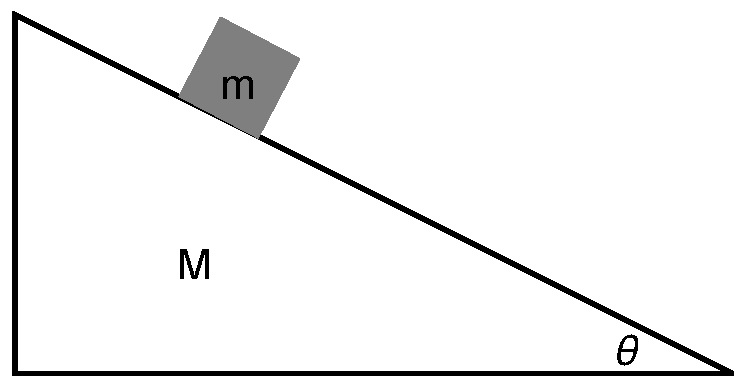
\includegraphics[width=5cm]{Diagram.pdf}
\centering
\end{figure}
\begin{enumerate}
\item What is the magnitude of the acceleration of mass $m$ down the inclinded plane?
    \begin{enumerate}
      \item $g\cos\theta$
      \item $g\sin\theta$
      \item $g\tan\theta$
      \item None of the above
    \end{enumerate}
  Hint: If you are deciding between (a), (b) and (c), please consider the limiting cases with $\theta=0$ and $\theta=\tfrac{\pi}{2}$.  
\item What is the most appropriate choice of coordinate system?
\item Find the equations of motion for the system.
\item What are acceleration of $m$ and $M$?
\item Discuss the accelerations in the following limiting cases.
    \begin{enumerate}
        \item $\theta=0$
        \item $M\rightarrow \infty$
        \item $M\rightarrow 0$
    \end{enumerate}
\item Find the magnitude of the normal force acting on mass $m$.
\item Discuss if the momentum of the system is conserved. Why or why not?
\item What is the mechanical energy of the system if the mass $m$ is initially at height of $h$ from the ground? Assume that the center of mass of $M$ is located at height $H$ from the ground.
\item When the mass $m$ reaches the bottom of the inclined plane, what is the mechanical energy of the system?
\item Is mechanical energy of this system  conserved? Discuss.
\end{enumerate}





\end{document}